\chapter{Domain Driven Design}
\section{Ubiquitous Language}
Es wurde sich bereits vor der Implementierung des Projektes gedanken über die Ubiquitous Language gemacht, wie in dem Commit \href{https://github.com/P3lina/ASE-Project/commit/0005472ee771b6231a118706708e1d19900958c2}{\textbf{0005472}} zu sehen ist. Für diese Vorgehensweise wurde sich bewusst entschieden, da die Namensgebung aller Klassen, Objekte, Variablen, Nachrichten usw. auf den Namen der Ubiquitous Language basieren.\\
Beispiele der Ubiquitous Language können auf der nächsten Seite gesehen werden.\\
\newcounter{ubctr}
\newcommand\unr{\stepcounter{ubctr}\arabic{ubctr}}

\newcolumntype{b}{X}
\newcolumntype{s}{>{\hsize=.5\hsize}X}

\begin{table}[H]
	\centering
	\begin{tabularx}{\textwidth}{rs|bb}
		& \textbf{Bezeichnung} & \textbf{Bedeutung} & \textbf{Begründung} \\
		\midrule
		\unr & \textbf{Match} & Ein Match ist das gesamte Spiel zwischen mehreren Spielern. Ein Spiel besteht aus mindestens einem Set. Ein Set besteht aus mindestens einem Leg. Ein Leg besteht aus mindestens einer Runde. & Vor allem für Dart-Neulingen könnten Dart Begriffe nicht geläufig sein und daher könnte ein Neuling davon ausgehen, dass ein Match gleich eneis Legs ist.\\
        \unr & \textbf{Score} & Der Score ist der Punktestand eines Spielers in einem Leg. Im klassischen Dart liegt er somit zwischen 0 und 501 Punkten. & Für den Score muss auch ein bestimmtes Wort festgelegt werden, damit die Verwendung von verschiedenen Begriffen, wie z.B. Points nicht zu Verwirrungen führen.\\
        \unr & \textbf{Dart} & Ein Dart ist ein Wurf auf die Dartscheibe. Ein Dart besteht aus einem Wert des Darts (\zB 60) und der Information, ob dieser Dart ein Doppelfeld getroffen hat, da dies wichtig ist für das Beenden eines Legs. & Es musste ein Begriff für einen einzelnen Dart festgelegt werden, damit er nicht mit dem Throw verwechselt wird.\\
        \unr & \textbf{Throw} & Ein Throw besteht aus drei geworfenen Darts auf die Dartscheibe. & Dieser Begriff wurde eingeführt, damit er nicht mit dem Einzelnen Dart-Wurf (Dart) verwechselt wird.\\
	\end{tabularx}
	\caption{Ubiquitous Language}
	\label{tab:ublang}
\end{table}
\section{Entities}
Eine Entity sei definiert über Identität, Lebenszyklus und Verhalten.\\
\textbf{Entity Match}:\\
\begin{figure}[ht]
    \centering
    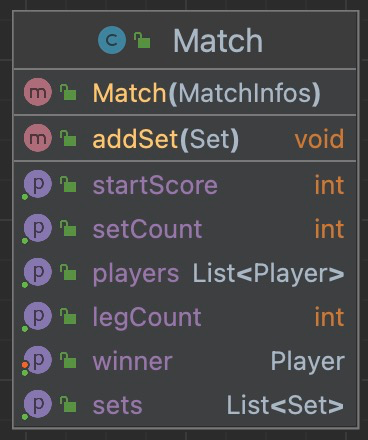
\includegraphics[width=0.4\textwidth]{Bilder/match.png}
    \caption{Match UML}
    \label{fig:match-uml}
\end{figure}
\begin{itemize}
    \item \textbf{Identität:} Jedes Match ist eindeutig und kann anhand einer Identität unterschieden werden. Auch wenn die Attribute (Spieler, Sets, etc.) des Matches sich ändern könnten, bleibt die Identität des Matches gleich. Die Identität könnte implizit durch eine Kombination der Attribute oder explizit durch eine eindeutige ID repräsentiert werden, falls nötig.
    \item Ein Match hat einen klaren Lebenszyklus und einen Zustand, der sich im Verlauf der Applikation ändert. Es wird initialisiert, Sets werden hinzugefügt, und schließlich wird ein Gewinner festgelegt.
    \item Das Match hat Methoden, die das Verhalten darstellen, wie ein Match manipuliert oder geändert werden kann.
\end{itemize}
\section{Value Objects}
In dieser Anwendung wurden keine vollwertigen Value Objects verwendet, da der Einsatz dieser nicht notwendig ist. Value Objects werden oft für elementare Werte verwendet, wie Geld oder eine Adresse, wobei solche Konzepte in der Anwendung nicht vorkommen.\\
Jedoch könnte ein abgewandeltes Objekt der Dart-Klasse als Value Object angesehen werden, da ein Dart Wurf insbesondere über sein Attribut \textit{points} definiert wird und somit zwei Dart Objekte mit der gleichen points-Anzahl als gleich angesehen werden können.
\section{Repositories}
Repositories sind besonders nützlich, wenn wiederholte Zugriffe auf bestimmte Objekte erforderlich sind, da sie das Definieren von spezifischem Suchverhalten für diese Objekte ermöglichen.\\
In dieser Anwendung wird immer nur am Ende eines Legs oder Sets auf andere Objekte zugegriffen. Zum Beispiel wird am Ende eines Legs auf die vorherigen Legs zugegriffen, um einen eventuellen Gewinner des Sets zu ermitteln. Da diese Zugriffe so selten geschehen, ist der Einsatz eines Repositories überflüssig und würde nur unnötig die Komplexität erhöhen.
\section{Aggregates}

Aggregates in \acf{DDD} sind Gruppen von assoziierten Objekten, die als Einheit behandelt werden, um die Konsistenz und Integrität der Geschäftsdaten zu gewährleisten. Jedes Aggregate hat eine sogenannte Root-Entität, die als Einstiegspunkt für die Interaktion mit dem Aggregate dient und die Kontrolle über den Lebenszyklus der inneren Objekte hat. Zugriffe auf innere Objekte eines Aggregats erfolgen in der Regel über die Root-Entität. So wird sichergestellt, dass Geschäftsregeln eingehalten werden und die Datenkonsistenz gewährleistet ist. Aggregates helfen, die Komplexität im Design zu reduzieren und die Isolation zwischen verschiedenen Teilen des Systems zu fördern. In diesem Projekt wurde kein spezifisches Aggregate implementiert, da der Entwurf so gewählt wurde, dass jedes Objekt für seine eigene Konsistenz zuständig ist.